\documentclass{article}
\usepackage{graphicx} % Required for inserting images
\usepackage{amssymb}
\usepackage{amsmath}
\usepackage{amsthm}
\usepackage{xcolor}
\usepackage{tikz}

\newtheorem{theorem}{Theorem}[section]
\newtheorem{corollary}[theorem]{Corollary}
\newtheorem{lemma}[theorem]{Lemma}
\newtheorem{definition}[theorem]{Definition}
\DeclareMathOperator*{\argmax}{arg\,max}
\DeclareMathOperator*{\argmin}{arg\,min}
\usepackage{hyperref}

\title{2026-Injectivity-Simplex-Method}
\author{kesterlester }
\date{June 2026} % Version before attempt to push back FCU/CU are sets idea

\begin{document}

\maketitle

\section{Definitions}
Where $n$ and $k$ appear they may always be assumed to be integers  greater than or equal to 2.

\phantomsection\label{def:sn}Let $s(n)$ be the set of length-$(n-1)$ ordered sequences of integers (without repeats) chosen from $[1,n]$.  Equivalently, each element of $s(n)$ is obtained by leaving out exactly one of the $n$ symbols and writing the remaining $n-1$ in some order (which symbol is left out will matter later).  For example $$s(3)=\{(1,2),(2,1),(1,3),(3,1),(2,3),(3,2)\}.$$
Clearly
$|s(n)| = {}^n P_{n-1} = n!.$

\phantomsection\label{def:oh}Let $oh(\vec v)$ be a function which takes an element of $\vec v\in s(n)$ to an ordered list of one-hot length-$n$ vectors (a \emph{one-hot} vector being one that is $1$ in a single position and $0$ everywhere else) defined using the Kronecker Delta as follows:
$$oh(\vec v) = (\vec o_1(\vec v), \vec o_2(\vec v), ..., \vec o_{n-1}(\vec v)) $$
with
$$(\vec o_i(\vec v))_j= \delta_{j \vec v_i}.$$
For example:
$oh((3,1)) = ( (0,0,1), (1,0,0))$
and
$oh((1,2)) = ( (1,0,0), (0,1,0))$.



\phantomsection\label{def:coh}Let $coh(\vec v)$ be a `cumulative' version of $oh(\vec v)$, that is to say:
$$(coh(\vec v))_i = \sum_{j=1}^i (oh(\vec v))_j.$$
For example: $coh((3,1)) = ( (0,0,1), (1,0,1))$
and
$coh((1,2)) = ( (1,0,0), (1,1,0))$.


\phantomsection\label{def:mat}Let $mat(\vec x,j)$ be a function which inserts the elements of $\vec x\in \mathbb Z^n$ into the $j$-th row of a $k \times n$ matrix which otherwise contains zeros.
    For example, if $n=4$ and $k=3$ we would have $$mat((2,4,3,9),2) = \begin{bmatrix} 0 & 0 & 0 & 0 \\ 2 & 3 & 4 & 9 \\ 0 & 0 &0 &0\end{bmatrix}.$$


\phantomsection\label{def:U}For $\vec v_i\in s(n)$ and $i \in [1,k]$  let $U(\vec v_1, \vec v_2, \ldots, \vec v_k)$ be the following set of $k\times n$-matrices:
$$ U(\vec v_1, \vec v_2, \ldots, \vec v_k)
=
\bigcup_{j=1}^k \bigcup_{m=1}^{n-1}\left\{ mat(coh(\vec v_j)_m, j) \right\}.
$$
For example, for $n=3$ and $k=2$ we would have
$$U((3,1), (1,2)) = \left\{
\begin{bmatrix}
0 & 0 & 1 \\
0 & 0 & 0
\end{bmatrix},
\begin{bmatrix}
1 & 0 & 1 \\
0 & 0 & 0
\end{bmatrix},
\begin{bmatrix}
0 & 0 & 0 \\
1 & 0 & 0
\end{bmatrix},
\begin{bmatrix}
0 & 0 & 0 \\
1 & 1 & 0 
\end{bmatrix}
\right\}
.$$
Note that $|U(\vec v_1, \vec v_2, \ldots, \vec v_k)|=(n-1)k$ and so if we wished to put the elements of the set $U(\vec v_1, \vec v_2, \ldots, \vec v_k)$ into some fixed order there would be $((n-1)k)!$ orderings available to us.

\phantomsection\label{def:ordering}For $p$ being an integer in $[1,((n-1)k)!]$ let $\vec U(\vec v_1, \vec v_2, \ldots, \vec v_k; p)$ be an ordering of the elements of $U(\vec v_1, \vec v_2, \ldots, \vec v_k)$.  (Think of $p$ simply as a \emph{name} for one particular ordering: there are $((n-1)k)!$ orderings, and $p$ ranges over labels for them.)  The only requirement on the ordering is that $$\left( 
\vec U(\vec v_1, \vec v_2, \ldots, \vec v_k; p) = 
\vec U(\vec v_1, \vec v_2, \ldots, \vec v_k; q) \right)
\iff
\left( p=q \right),
$$
i.e.~that distinct values of $p$ select different permuations.
%
For example, it might be the case that 
$$\vec U((3,1), (1,2); 1) = \left(
\begin{bmatrix}
0 & 0 & 1 \\
0 & 0 & 0
\end{bmatrix},
\begin{bmatrix}
1 & 0 & 1 \\
0 & 0 & 0
\end{bmatrix},
\begin{bmatrix}
0 & 0 & 0 \\
1 & 0 & 0
\end{bmatrix},
\begin{bmatrix}
0 & 0 & 0 \\
1 & 1 & 0 
\end{bmatrix}
\right)$$
while
$$\vec U((3,1), (1,2); 2) = \left(
\begin{bmatrix}
0 & 0 & 1 \\
0 & 0 & 0
\end{bmatrix},
\begin{bmatrix}
1 & 0 & 1 \\
0 & 0 & 0
\end{bmatrix},
\begin{bmatrix}
0 & 0 & 0 \\
1 & 1 & 0 
\end{bmatrix},
\begin{bmatrix}
0 & 0 & 0 \\
1 & 0 & 0
\end{bmatrix}
\right).$$

\phantomsection\label{def:CU}Let $C\vec U$ be a cumulative version of $\vec U$, i.e.~for $i$ in $[1,(n-1)k]$ we define
$$\left( C\vec U(\vec v_1, \vec v_2, \ldots, \vec v_k; p)\right)_i
=
\sum_{j=1}^{i}\left(
\vec U(\vec v_1, \vec v_2, \ldots, \vec v_k; p) \right)_j.
$$
For example, if
$$\vec U((3,1), (1,2); 3) = \left(
\begin{bmatrix}
0 & 0 & 1 \\
0 & 0 & 0
\end{bmatrix},
\begin{bmatrix}
0 & 0 & 0 \\
1 & 1 & 0 
\end{bmatrix},
\begin{bmatrix}
1 & 0 & 1 \\
0 & 0 & 0
\end{bmatrix},
\begin{bmatrix}
0 & 0 & 0 \\
1 & 0 & 0
\end{bmatrix}
\right)$$
then
$$C\vec U((3,1), (1,2); 3) = \left(
\begin{bmatrix}
0 & 0 & 1 \\
0 & 0 & 0
\end{bmatrix},
\begin{bmatrix}
0 & 0 & 1 \\
1 & 1 & 0 
\end{bmatrix},
\begin{bmatrix}
1 & 0 & 2 \\
1 & 1 & 0
\end{bmatrix},
\begin{bmatrix}
1 & 0 & 2 \\
2 & 1 & 0
\end{bmatrix}
\right).$$

\phantomsection\label{def:FCU}Let a `filter', $\vec f$, be a length-$(n-1)k$-vector consisting of only zeros or ones that can `hide' elements of $C\vec U$ to make a filtered ordered list
$FC\vec U$ as follows:
$$
   \left( FC\vec U(\vec v_1, \vec v_2, \ldots, \vec v_k; p,\vec f) \right)_i =
    \begin{cases}
    \left( C\vec U(\vec v_1, \vec v_2, \ldots, \vec v_k; p) \right)_i \qquad & \text{if $(\vec f)_i = 1$},\\
    Null & \text{otherwise.}
    \end{cases}
$$
For example, if the filter is $\vec f=(1,1,0,1)$ and 
\begin{align}C\vec U((3,1), (1,2); 3) = \left(
\begin{bmatrix}
0 & 0 & 1 \\
0 & 0 & 0
\end{bmatrix},
\begin{bmatrix}
0 & 0 & 1 \\
1 & 1 & 0 
\end{bmatrix},
\begin{bmatrix}
1 & 0 & 2 \\
1 & 1 & 0
\end{bmatrix},
\begin{bmatrix}
1 & 0 & 2 \\
2 & 1 & 0
\end{bmatrix}
\right)\label{eq:cu3example}
\end{align}
then
$$FC\vec U((3,1), (1,2); 3,(1,1,0,1))
=
\left(
\begin{bmatrix}
0 & 0 & 1 \\
0 & 0 & 0
\end{bmatrix},
\begin{bmatrix}
0 & 0 & 1 \\
1 & 1 & 0 
\end{bmatrix},
Null,
\begin{bmatrix}
1 & 0 & 2 \\
2 & 1 & 0
\end{bmatrix}
\right).
$$

\phantomsection\label{def:clean}Finally, let $clean(\vec L)$ be a function which takes an ordered list $\vec L$ (some of whose entries may be $Null$) and returns the shorter list obtained by deleting every $Null$ and closing up the gaps, leaving the surviving matrices in their original relative order.
For example, continuing the case above,
$$
clean\left( FC\vec U((3,1), (1,2); 3,(1,1,0,1)) \right)
=
\left(
\begin{bmatrix}
0 & 0 & 1 \\
0 & 0 & 0
\end{bmatrix},
\begin{bmatrix}
0 & 0 & 1 \\
1 & 1 & 0
\end{bmatrix},
\begin{bmatrix}
1 & 0 & 2 \\
2 & 1 & 0
\end{bmatrix}
\right).
$$
Note that $clean$ discards the knowledge of \emph{where} the $Null$s sat: it preserves the surviving matrices' order relative to one another, but not the absolute positions ($1,2,3,\ldots$) they originally occupied in the list.

\subsection*{A useful observation: $C\vec U$ and $FC\vec U$ are really sets}

Each cumulative matrix quietly records its own position.  The largest entry in a
row counts how many of that row's pieces have been added in so far, so summing the
largest entry over all rows returns the matrix's position in the list.  For the
third matrix of $C\vec U((3,1),(1,2);3)$ above,
\[
m_3=\begin{bmatrix}1&0&2\\1&1&0\end{bmatrix},
\qquad
\underbrace{\max(1,0,2)}_{2}+\underbrace{\max(1,1,0)}_{1}=3,
\]
which is indeed where it sits.  Consequently the order in which the matrices of
$C\vec U$ are listed -- and, for $FC\vec U$, where the $Null$s fall -- can always be
reconstructed from the matrices themselves.  \textbf{We may therefore treat
$C\vec U$ and $FC\vec U$ as \emph{sets} of matrices}, and will do so freely below;
nothing we ask of them depends on their stored order.  (The intermediate object
$\vec U$ is different -- its plain one-hot matrices do not betray their positions --
so for $\vec U$ the listed order is genuine.)

\subsection{Placing columns into canonical orders -- (a.k.a.~column `sorting')}
\label{subsec:sorting}

\phantomsection\label{def:colperm}Before describing the two sorting processes we need one piece of notation.  A
\emph{permutation} $\sigma$ of $[1,n]$ is a relabelling of the column positions
$\{1,2,\ldots,n\}$ -- a one-to-one correspondence of that set with itself.  (The set
of all $n!$ such permutations is written $S_n$.)  For a
$k\times n$ matrix $m$, let $colPerm(m,\sigma)$ denote the matrix obtained by moving
the contents of column $c$ to column $\sigma(c)$, simultaneously in every row.  For
example, if $\sigma$ sends $1\mapsto2,\ 2\mapsto3,\ 3\mapsto1$ then
$$
colPerm\left(\begin{bmatrix}1&0&2\\1&1&0\end{bmatrix},\sigma\right)
=\begin{bmatrix}2&1&0\\0&1&1\end{bmatrix}
$$
(the old column $1$ has gone to position $2$, column $2$ to position $3$, and column
$3$ to position $1$).

Suppose now that $\vec L=(m_1, m_2, \ldots, m_{(n-1)k})$ is an ordered list wherein
each element $m_u$ is either a $k\times n$-matrix or a $Null$ value (representing a
filtered-away matrix).  One can imagine two different (but related) column
re-ordering processes which could be applied to the matrices in $\vec L$.  Call
these:
\begin{enumerate}
\item
Local column sorting, and
\item
Global column sorting.
\end{enumerate}

\paragraph{Local column sorting.}
Here each matrix is tidied \emph{on its own}.  We suppose we have some fixed rule
$canon(\cdot)$ that takes a matrix to a chosen ``standard'' column-ordering of it,
and we apply it to each matrix independently:
$$localSort(\vec L) = \left(
canon(m_1), canon(m_2), \ldots, canon(m_{(n-1)k})
\right).
$$
We deliberately do \emph{not} pin down which standard ordering $canon$ produces,
because nothing in this document depends on the choice: a companion document that
uses this machinery is free to pick its own rule, and may even change it from time
to time.  The \emph{only} property we ever require of $canon$ is that it be a
genuine canonical form -- that it give two matrices the same output exactly when
they are column-reorderings of one another:
\begin{align}
canon(a)=canon(b)
\quad\iff\quad
a=colPerm(b,\sigma)\ \text{for some }\sigma.
\label{eq:canonprop}
\end{align}
(For concreteness, one rule obeying \eqref{eq:canonprop} is: read each matrix's
entries off in a fixed order, say row by row, and among all $n!$ column-reorderings
keep the one whose readout is alphabetically smallest.  But this is only an
\emph{example}; any rule satisfying \eqref{eq:canonprop} serves equally well, and we
rely on no other feature of it.)

\paragraph{Global column sorting.}
Here, in contrast, a \emph{single} column permutation $\sigma$ must be applied
synchronously to \emph{all} the matrices at once, and only then is the whole list
tidied to a standard form.  We suppose we have some fixed rule $globalSort(\cdot)$
that selects a standard representative from among all the lists
$$
\left(
colPerm(m_1, \sigma), colPerm(m_2, \sigma), \ldots, colPerm(m_{(n-1)k},\sigma)
\right),
\qquad \sigma\in S_n,
$$
reachable by re-shuffling the columns of every matrix by one common $\sigma$.  As
with $canon$ we do not commit to \emph{how} the representative is chosen; the only
property we require is the exact analogue of \eqref{eq:canonprop}, one level up --
that two lists receive the same $globalSort$ precisely when one can be turned into
the other by a single common column permutation:
\begin{align}
\begin{split}
globalSort(\vec L)=globalSort(\vec L')
\iff{}& m'_i=colPerm(m_i,\sigma)\\[-2pt]
& \text{for all }i,\ \text{for one common }\sigma.
\end{split}
\label{eq:globalprop}
\end{align}
The contrast between the two is the whole point.  Local sorting is allowed a
\emph{different} reshuffle for each matrix; global sorting must make \emph{one}
reshuffle serve them all.  Global agreement is therefore the harder thing to
achieve, and the question of Section~\ref{sec:problem} is whether it is nonetheless
forced by local agreement.

%======================================================================
%  NEW SELF-CONTAINED SOLUTION  (Sections 2 onwards)
%======================================================================

\section{The problem we really want to solve}
\label{sec:problem}

Everything in Section~1 was scaffolding.  Here is the question we actually
care about.

\phantomsection\label{def:config}Throughout, fix two \emph{configurations}
\[
\vec v=(\vec v_1,\ldots,\vec v_k)
\qquad\text{and}\qquad
\vec u=(\vec u_1,\ldots,\vec u_k),
\qquad \vec v_j,\vec u_j\in s(n).
\]
Each is just a list of $k$ sequences of the kind defined in Section~1.  Think of
$\vec v$ as one ``experiment'' and $\vec u$ as another, and the question we ask is
always: \emph{can we tell these two experiments apart} after we have processed
them in the elaborate way Section~1 describes?

\medskip
\noindent\textbf{The problem.}
We wish to know whether, for \emph{all} filters $\vec f$ and \emph{all} orderings
$p$ and $q$,
\begin{gather}
\Bigl(
globalSort\bigl(clean(FC\vec U(\vec v;p,\vec f))\bigr)
=
globalSort\bigl(clean(FC\vec U(\vec u;q,\vec f))\bigr)
\Bigr)
\nonumber\\[2pt]
\iff
\label{eq:mainproblem}\\[2pt]
\Bigl(
localSort\bigl(clean(FC\vec U(\vec v;p,\vec f))\bigr)
=
localSort\bigl(clean(FC\vec U(\vec u;q,\vec f))\bigr)
\Bigr).
\nonumber
\end{gather}
Either we need a proof that \eqref{eq:mainproblem} always holds, or a counterexample.

\medskip
\noindent\textbf{What the two sides mean, in words.}
Both sides take the same raw ingredients, filter them with the same $\vec f$,
throw away the gaps, and then try to line up the columns of the resulting
matrices into a canonical order.  They differ only in \emph{how much freedom} the
column re-ordering is given (this is the distinction between \emph{local} and
\emph{global} column sorting drawn at the end of Section~1):
\begin{itemize}
  \item \textbf{localSort} canonicalises \emph{each matrix on its own}: every
        matrix may choose its own column permutation.
  \item \textbf{globalSort} must canonicalise \emph{all the matrices at once}
        using a \emph{single} column permutation applied to every matrix
        simultaneously.
\end{itemize}
Global agreement is therefore the stronger, more demanding statement.  The
content of \eqref{eq:mainproblem} is the claim that, surprisingly, the weaker
``each-matrix-separately'' notion of agreement is already enough to force the
stronger ``all-at-once'' one.  We will prove that it is.

\begin{theorem}\label{thm:main}
For every pair of configurations $\vec v,\vec u$, every filter $\vec f$, and all
orderings $p,q$, the biconditional \eqref{eq:mainproblem} holds.
\end{theorem}

\subsection*{First simplification: the lists are secretly sets}

The statement \eqref{eq:mainproblem} looks forbidding because of the four wrappers
($globalSort$/$localSort$, $clean$, $FC\vec U$, and the orderings $p,q$).  The
first thing to do is to dissolve most of them.

The key was already noticed in Section~1: \emph{a cumulative matrix records its own
position in the list}.  If $m_i$ is the $i$-th cumulative matrix, then summing the
largest entry in each of its $k$ rows returns $i$:
\begin{align}
i=\sum_{r=1}^{k}\ \max_{c\in[1,n]}\,(m_i)_{rc}.
\label{eq:recovery}
\end{align}
For example, with $C\vec U((3,1),(1,2);3)$ from Section~1 the third matrix is
\[
m_3=\begin{bmatrix}1&0&2\\1&1&0\end{bmatrix},
\qquad
\underbrace{\max(1,0,2)}_{2}+\underbrace{\max(1,1,0)}_{1}=3,
\]
which is exactly its position.

Two consequences follow, and together they remove three of the four wrappers.

\begin{itemize}
  \item \textbf{Cleaning loses nothing.}  Because each surviving matrix announces
        its own absolute position through \eqref{eq:recovery}, the positions of the
        discarded $Null$s can be reconstructed from the survivors alone.  Whatever
        information $clean$ appears to destroy was never really lost.
  \item \textbf{Order is redundant.}  For the same reason, the order in which the
        matrices are listed can always be recovered from the matrices themselves.
        So we may treat each of $C\vec U$, $FC\vec U$ and its cleaned form not as an
        \emph{ordered list} but simply as a \emph{set} of matrices.
\end{itemize}

\begin{corollary}\label{cor:sets}
$C\vec U(\vec v;p)$ and $FC\vec U(\vec v;p,\vec f)$ may be regarded as
\emph{sets} of matrices: the order intended for their elements is always
recoverable from the elements themselves via \eqref{eq:recovery}.  Consequently
$clean$ has no effect on the underlying set, and the equalities in
\eqref{eq:mainproblem} are equalities of \emph{sets} of matrices.
\end{corollary}

There is one subtlety to check before we lean on this.  Both $localSort$ and
$globalSort$ act by \emph{permuting columns}, and permuting the columns of a row
never changes \emph{which numbers} appear in that row -- only their left-to-right
arrangement.  In particular the largest entry of each row is unchanged, so the
position formula \eqref{eq:recovery} keeps working \emph{after} sorting as well as
before.  Hence a sorted, cleaned list is still recoverable from its set of
matrices, and ``the two sorted lists are equal'' means exactly ``the two sets of
sorted matrices are equal''.  This is what lets us speak of sets from now on.

\medskip
\noindent\textbf{What remains.}  Stripped of $clean$ and of the ordering bookkeeping,
the problem is this.  Each side produces a \emph{set of matrices}.  We must compare
\begin{itemize}
  \item the set obtained by sorting \emph{each matrix's columns independently}
        ($localSort$), against
  \item the set obtained by sorting \emph{all matrices' columns with one common
        permutation} ($globalSort$),
\end{itemize}
and show the two notions of ``the $\vec v$-set equals the $\vec u$-set'' coincide.
The rest of the document does this.  The plan is:
\begin{itemize}
  \item[\S\ref{sec:snapshots}] introduces a cleaner name -- a \emph{snapshot} --
        for the matrices that appear, indexed not by a position but by the set of
        ingredients that built it;
  \item[\S\ref{sec:remember}] proves that a snapshot \emph{remembers exactly which
        ingredients built it} (formula \eqref{eq:recovery} is the shallow end of
        this);
  \item[\S\ref{sec:align}] settles, for a single snapshot, exactly when the
        $\vec v$-version and $\vec u$-version are column re-orderings of each other;
  \item[\S\ref{sec:solution}] assembles these into a proof of
        Theorem~\ref{thm:main}.
\end{itemize}


\section{Snapshots}
\label{sec:snapshots}

This section renames the objects of Section~1 in a way that makes the proof short.
No new mathematics happens here; we are only choosing better bookkeeping.

\subsection*{Slots and slot-sets}

The raw ingredients of Section~1 -- the elements of the set
$U(\vec v_1,\ldots,\vec v_k)$ -- are indexed by two numbers: a \emph{row}
$j\in[1,k]$ and a \emph{level} $m\in[1,n-1]$.  Call the pair $(j,m)$ a \emph{slot}.
There are exactly $L=(n-1)k$ slots, one for each ingredient.  The slot $(j,m)$
names the ingredient ``put the cumulative one-hot $coh(\vec v_j)_m$ into row $j$,
zeros elsewhere''.

\phantomsection\label{def:slot}A \emph{slot-set} $Q$ is just any set of slots, $Q\subseteq\{(j,m)\}$.  Given a
slot-set $Q$, gather for each row $j$ the levels it contains:
\[
A_j(Q)=\{\,m:(j,m)\in Q\,\}\subseteq[1,n-1].
\]
So $Q$ is completely described by its $k$ level-sets $A_1(Q),\ldots,A_k(Q)$.

\subsection*{Prefix sets}

\phantomsection\label{def:prefix}For a sequence $\vec w\in s(n)$ and a level $m$, write
\[
P_m(\vec w)=\{\vec w_1,\vec w_2,\ldots,\vec w_m\}
\]
for the \emph{prefix set}: the set of the first $m$ symbols of $\vec w$ (forgetting
their order).  Because $\vec w$ has no repeats, these grow one symbol at a time and
are \emph{nested},
\[
P_1(\vec w)\subset P_2(\vec w)\subset\cdots\subset P_{n-1}(\vec w).
\]
The cumulative one-hot vector $coh(\vec w)_m$ from Section~1 is precisely the
\emph{indicator} of $P_m(\vec w)$ -- the length-$n$ row of $0$s and $1$s with a $1$
in column $c$ exactly when $c\in P_m(\vec w)$.  For instance with $\vec w=(3,1)$ we
have $P_1=\{3\}$, $P_2=\{3,1\}$, and the indicators $(0,0,1)$ and $(1,0,1)$.

\subsection*{The snapshot matrix}

\begin{definition}\label{def:snapshot}
For a configuration $\vec v=(\vec v_1,\ldots,\vec v_k)$ and a slot-set $Q$, the
\emph{snapshot} $M^{\vec v}(Q)$ is the $k\times n$ matrix whose row $j$ is the sum
of the indicators of the prefixes named by $Q$:
\[
\bigl(M^{\vec v}(Q)\bigr)_{\text{row }j}
=\sum_{m\in A_j(Q)} coh(\vec v_j)_m .
\]
\end{definition}

This is nothing more than ``add up the ingredients whose slots lie in $Q$''.  The
link to Section~1 is immediate: if $Q_i$ denotes the set of the \emph{first $i$
slots} in an ordering $p$, then $M^{\vec v}(Q_i)$ is exactly the $i$-th cumulative
matrix of $C\vec U(\vec v;p)$.  The word ``snapshot'' is apt: $M^{\vec v}(Q_i)$ is
a frozen moment of the running total after $i$ steps.  But the definition makes
sense for \emph{any} slot-set $Q$, prefix or not, and that extra generality costs
nothing.

\medskip
\noindent\textit{A worked snapshot.}  Take $n=3$, $k=2$, $\vec v=((3,1),(1,2))$ --
the running example of Section~1 -- and the slot-set
$Q=\{(1,1),(1,2),(2,2)\}$, so that $A_1(Q)=\{1,2\}$ and $A_2(Q)=\{2\}$.  Row $1$ is
$coh(\vec v_1)_1+coh(\vec v_1)_2=(0,0,1)+(1,0,1)=(1,0,2)$, and row $2$ is
$coh(\vec v_2)_2=(1,1,0)$.  Thus
\[
M^{\vec v}(Q)=\begin{bmatrix}1&0&2\\[1pt]1&1&0\end{bmatrix}.
\]

\subsection*{The values depend on $Q$ alone; the configuration only moves them around}

\phantomsection\label{def:wr}We first fix one small piece of notation.  For a sequence $\vec w\in s(n)$ write
$(\vec w)_r$ for its $r$-th entry -- the symbol in position $r$ -- so that
``column $(\vec w)_r$'' means the column belonging to that symbol.  As $r$ runs
$1,\ldots,n-1$ these name the $n-1$ columns that $\vec w$ uses; the single left-out
symbol owns the one remaining column.

Here is the observation that makes the whole problem tractable.  Look at row $j$ of
a snapshot.  The prefixes are nested, so the entry in column $(\vec v_j)_r$ simply
counts how many of the chosen levels reach that far:
\[
\bigl(M^{\vec v}(Q)\bigr)_{j,\,(\vec v_j)_r}
=\#\{\,m\in A_j(Q): m\ge r\,\},
\]
and the one column belonging to the omitted symbol gets a $0$ (recall that each
sequence $\vec v_j$ lists only $n-1$ of the $n$ symbols, so exactly one symbol --
and hence one column -- never appears).  The crucial point:
the \emph{multiset of values} appearing in row $j$ -- namely
$\{\#\{m\in A_j(Q):m\ge r\}: r\}$ together with the extra $0$ -- depends only on
$A_j(Q)$, \textbf{not} on the sequence $\vec v_j$.  \label{def:multiset}(A \emph{multiset} is a
collection in which repeats are allowed and counted but order is ignored: thus
$\{2,1,0\}$ and $\{0,1,2\}$ are the same multiset, whereas $\{1,1,0\}$ differs from
$\{1,0\}$.)  The sequence decides only \emph{which column} each value lands in.

\medskip
\noindent\textit{Same values, different columns.}  With $A_1(Q)=\{1,2\}$ the row-$1$
values are $\#\{m\ge1\}=2$, $\#\{m\ge2\}=1$, plus a $0$: the multiset $\{2,1,0\}$,
whatever the sequence.  If $\vec v_1=(3,1)$ then $2$ goes to column $3$, $1$ to
column $1$, $0$ to column $2$, giving row $(1,0,2)$.  If instead the sequence were
$(2,3)$ the \emph{same} values $\{2,1,0\}$ would sit in different columns, giving
row $(0,2,1)$.  Same contents; different arrangement.

This single fact -- \emph{contents fixed by $Q$, arrangement fixed by the
sequence} -- is the seed of both halves of the proof.  Reading off the contents
will tell us $Q$ (Section~\ref{sec:remember}); comparing the arrangements will tell
us when two configurations agree (Section~\ref{sec:align}).


\section{A snapshot remembers how it was built}
\label{sec:remember}

We now prove that a snapshot matrix secretly carries a complete record of the
slot-set that produced it.  Formula \eqref{eq:recovery} read off one number from
each row; here we read off the whole row.

\begin{lemma}\label{lem:recover}
Fix a row $j$ and let $A=A_j(Q)$.  From the multiset of entries in row $j$ of
$M^{\vec v}(Q)$ one can recover the set $A$ completely, and the recovery does not
use the sequence $\vec v_j$.  Explicitly, for every integer $t\ge1$,
\[
\#\{\,c:\bigl(M^{\vec v}(Q)\bigr)_{j,c}\ge t\,\}
=
\bigl(\text{the $t$-th largest element of }A\bigr),
\]
and this count is $0$ once $t>|A|$.  Hence, listing $A=\{a_1>a_2>\cdots>a_{|A|}\}$,
the numbers $a_1,a_2,\ldots$ are read straight off the row.
\end{lemma}

\begin{proof}
By the displayed formula of Section~\ref{sec:snapshots}, the entry in column
$(\vec v_j)_r$ is $\#\{m\in A:m\ge r\}$ (and the absent column is $0$).  Such
an entry is $\ge t$ precisely when its position $r$ satisfies $r\le a_t$, where $a_t$
is the $t$-th largest element of $A$; there are exactly $a_t$ such positions.  So the
number of columns with entry $\ge t$ equals $a_t$.  These counts mention only $A$,
never the sequence, and running $t=1,2,\ldots$ recovers $a_1,a_2,\ldots$, i.e.\ all
of $A$.
\end{proof}

\noindent\textit{Example.}  Row $1$ of the snapshot above was $(1,0,2)$.  Columns
with entry $\ge1$: two of them, so $a_1=2$; with entry $\ge2$: one, so $a_2=1$;
with entry $\ge3$: none, so we stop.  Thus $A_1(Q)=\{2,1\}=\{1,2\}$, exactly the
levels we put in -- recovered from the row alone, with no reference to the sequence
$(3,1)$.

The reading is easiest to see as a picture, and is clearer in a less trivial case.
Suppose some snapshot row -- in an example with $n=6$, so columns
$c_1,\ldots,c_6$ -- reads $(0,3,3,1,1,2)$.  Draw its entries as bar heights and rule
in the thresholds $t=1,2,3$:
\begin{center}
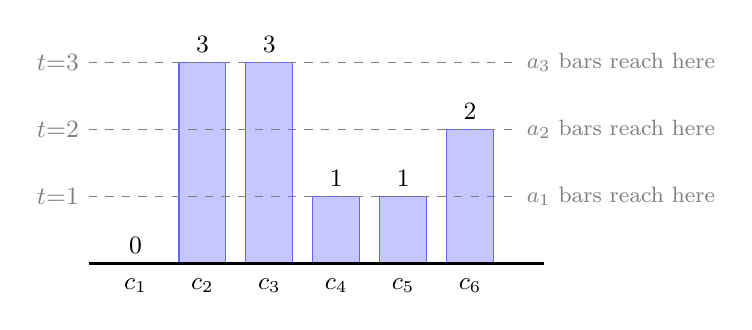
\begin{tikzpicture}[scale=0.85, every node/.style={font=\small}]
  \foreach \i/\h in {1/0,2/3,3/3,4/1,5/1,6/2}{
    \ifnum\h>0
      \fill[blue!22,draw=blue!60] (\i-0.35,0) rectangle (\i+0.35,\h);
    \fi
    \node[below] at (\i,-0.08) {$c_{\i}$};
    \node[above] at (\i,\h) {$\h$};
  }
  \draw[thick] (0.3,0) -- (7.1,0);
  \foreach \t in {1,2,3}{
    \draw[dashed,gray] (0.3,\t) -- (6.7,\t);
    \node[gray,left] at (0.3,\t) {$t{=}\t$};
    \node[gray,right,font=\footnotesize] at (6.7,\t) {$a_{\t}$ bars reach here};
  }
\end{tikzpicture}
\end{center}
Counting the bars that reach each dashed line gives $a_1=5$ (entries $\ge1$),
$a_2=3$ (entries $\ge2$), $a_3=2$ (entries $\ge3$), and nothing reaches higher; so
the row must have been built from the level-set $A=\{5,3,2\}$.  Notice we never
needed to know \emph{which} sequence produced the row: the bar heights alone give
back $A$.

Two corollaries do all the work later.

\begin{corollary}[the whole slot-set is remembered]\label{cor:wholeQ}
The entire slot-set $Q$ can be recovered from the matrix $M^{\vec v}(Q)$: apply
Lemma~\ref{lem:recover} to each row $j$ to get $A_j(Q)$, then
$Q=\{(j,m):m\in A_j(Q)\}$.  In particular two snapshots built from
\emph{different} slot-sets are different matrices, whatever the configurations.
\end{corollary}

\begin{corollary}[remembering survives column sorting]\label{cor:survives}
Permuting the columns of a snapshot does not change any row's multiset of entries,
so $Q$ is still recoverable afterwards.  In particular
$Q$ can be read from $localSort$'s or $globalSort$'s output just as from the
original.
\end{corollary}

\noindent Formula \eqref{eq:recovery} is just the special case $t=1$: the count of
nonzero entries in row $j$ is $a_1=|A_j(Q)|$, and summing over rows gives
$|Q|$, the position.  Lemma~\ref{lem:recover} simply keeps reading down the row
instead of stopping at the top.

These corollaries are exactly what we need to defeat the two ``extra freedoms'' in
the problem.  Corollary~\ref{cor:survives} (with $t=1$) was the content of
Corollary~\ref{cor:sets}: it lets us ignore $clean$ and ordering and work with
sets.  Corollary~\ref{cor:wholeQ} will let us ignore the fact that the two sides
may use \emph{different} orderings $p\ne q$: if a $\vec v$-snapshot and a
$\vec u$-snapshot ever match (even after independent column sorting) they must have
been built from one and the same slot-set.


\section{When are two snapshots the same up to column order?}
\label{sec:align}

Fix a single slot-set $Q$ and compare the two snapshots $M^{\vec v}(Q)$ and
$M^{\vec u}(Q)$ built from it.  By the previous section they have, row by row, the
same multiset of values; they can differ only in \emph{which columns} hold those
values.  When is one merely a column-rearrangement of the other?

\subsection*{Vocabulary: permutations and column equivalence}

\phantomsection\label{def:colequiv}Recall from Section~1 that a \emph{permutation} $\sigma\in S_n$ relabels the columns
$[1,n]$, and that $colPerm(M,\sigma)$ is the matrix got by sending the contents of
column $c$ to column $\sigma(c)$ in every row.  Two matrices are
\emph{column-equivalent}, written $M\sim M'$, if some single $\sigma$ achieves
$colPerm(M,\sigma)=M'$ -- that is, if one is a column-rearrangement of the other.
This is exactly the relation that $canon$ detects: by \eqref{eq:canonprop},
$canon(M)=canon(M')$ iff $M\sim M'$.

\subsection*{Aligning the revealed prefixes}

Recall (Section~\ref{sec:snapshots}) that reading row $j$ of $M^{\vec v}(Q)$ at
``height $\ge t$'' returns a prefix set $P_{a_t}(\vec v_j)$.  As $t$ ranges over
$1,\ldots,|A_j(Q)|$ these are precisely the prefixes
$\{P_m(\vec v_j):m\in A_j(Q)\}$.  So a snapshot is best thought of as a device that
\emph{displays}, in each row, a nested stack of prefix sets -- one prefix for each
level in $A_j(Q)$.  Lining up two snapshots column-by-column therefore means lining
up these displayed prefixes.  Define\phantomsection\label{def:sigma}
\[
\Sigma(Q)=\bigl\{\,\sigma\in S_n:\ \sigma\bigl(P_m(\vec v_j)\bigr)=P_m(\vec u_j)
\ \text{for all }j\in[1,k],\ m\in A_j(Q)\,\bigr\},
\]
the relabellings that carry every prefix revealed by $\vec v$ onto the matching
prefix revealed by $\vec u$.  (Here $\sigma(S)$ means $\{\sigma(c):c\in S\}$.)

\begin{lemma}[alignment]\label{lem:align}
$M^{\vec v}(Q)\sim M^{\vec u}(Q)$ if and only if $\Sigma(Q)\neq\varnothing$.  More
precisely, $\Sigma(Q)$ is \emph{exactly} the set of column permutations $\sigma$
with $colPerm(M^{\vec v}(Q),\sigma)=M^{\vec u}(Q)$.
\end{lemma}

\begin{proof}
A matrix of non-negative integers is determined by its family of
``level sets'' $\{c:\text{entry}\ge t\}$ in each row (the set of columns whose entry
clears height $t$, for each threshold $t=1,2,\ldots$).  In row $j$ of
$M^{\vec v}(Q)$ that level set is the prefix $P_{a_t}(\vec v_j)$, with $a_t$ the
$t$-th largest element of $A_j(Q)$; and crucially $A_j(Q)$ is the \emph{same} on
the $\vec u$-side, so the thresholds $a_t$ match.  Applying $colPerm(\cdot,\sigma)$
sends each level set $S$ to $\sigma(S)$.  Hence $colPerm(M^{\vec v}(Q),\sigma)$
equals $M^{\vec u}(Q)$ exactly when, in every row $j$ and at every threshold,
$\sigma\bigl(P_{a_t}(\vec v_j)\bigr)=P_{a_t}(\vec u_j)$ -- that is, when
$\sigma(P_m(\vec v_j))=P_m(\vec u_j)$ for all $j$ and all $m\in A_j(Q)$, which is the
definition of $\sigma\in\Sigma(Q)$.
\end{proof}

\noindent\textit{Example (a relabelling, and a non-relabelling).}  Keep
$n=3$, $k=2$, $\vec v=((3,1),(1,2))$ and $Q=\{(1,1),(1,2),(2,2)\}$, so
\[
M^{\vec v}(Q)=\begin{bmatrix}1&0&2\\1&1&0\end{bmatrix}.
\]
Take $\vec u=((2,3),(3,1))$, obtained from $\vec v$ by the single relabelling
$\sigma:1\mapsto3,\ 2\mapsto1,\ 3\mapsto2$ applied to every symbol.  Then
\[
M^{\vec u}(Q)=\begin{bmatrix}0&2&1\\1&0&1\end{bmatrix}
=colPerm\!\left(M^{\vec v}(Q),\sigma\right),
\]
so $M^{\vec v}(Q)\sim M^{\vec u}(Q)$ and indeed $\sigma\in\Sigma(Q)$: one
relabelling reorders the columns of \emph{both} rows at once.  By contrast take
$\vec w=((1,3),(2,1))$, which is \emph{not} a relabelling of $\vec v$.  Lining up
the displayed prefixes would force, from row $1$ at level $1$, that
$\sigma(\{3\})=\{1\}$, i.e.\ $\sigma(3)=1$; yet row $2$ at level $2$ forces
$\sigma(\{1,2\})=\{2,1\}$, i.e.\ $\sigma$ maps $\{1,2\}$ onto $\{1,2\}$ -- so the
symbol $1$ would have to be the image of $3$ \emph{and} of one of $1,2$ at once,
which no bijection allows.  Hence $\Sigma(Q)=\varnothing$ and the two snapshots are
genuinely different no matter how their columns are shuffled.

\subsection*{The richer the snapshot, the fewer alignments survive}

A snapshot built from more slots displays more prefixes, hence imposes more
constraints on an aligning $\sigma$.  This monotonicity is the engine of the whole
argument.

\begin{corollary}[monotonicity]\label{cor:mono}
If $Q'\subseteq Q$ then $\Sigma(Q)\subseteq\Sigma(Q')$.
\end{corollary}

\begin{proof}
A smaller slot-set has smaller level-sets, $A_j(Q')\subseteq A_j(Q)$ for every $j$.
The conditions defining $\Sigma(Q')$ are therefore a sub-list of those defining
$\Sigma(Q)$.  Adding requirements can only shrink the solution set, so any
$\sigma$ in $\Sigma(Q)$ already lies in $\Sigma(Q')$.
\end{proof}


\section{Putting it together}
\label{sec:solution}

We can now prove Theorem~\ref{thm:main}.  Fix $\vec v,\vec u,\vec f,p,q$.

\subsection*{The retained slot-sets}

\phantomsection\label{def:retained}Let $Q^p_i$ be the set of the first $i$ slots in ordering $p$.  These are
\emph{nested}, $Q^p_1\subset Q^p_2\subset\cdots$, so they form what is called a
\emph{chain}: any two of them are comparable, one contained in the other.  The
filter $\vec f$ keeps some of them; write
\[
\mathcal R_{\vec v}=\{\,Q^p_i:(\vec f)_i=1\,\},
\qquad
\mathcal R_{\vec u}=\{\,Q^q_i:(\vec f)_i=1\,\}
\]
for the families of \emph{retained} slot-sets on the two sides.  Each is a chain
(a sub-collection of a chain), so if non-empty it has a largest member.

By Corollary~\ref{cor:sets} the cleaned, sorted output of each side is just a
\emph{set} of matrices, namely
\[
\{\,canon\,M^{\vec v}(Q):Q\in\mathcal R_{\vec v}\,\}
\quad\text{(local, $\vec v$ side)},
\]
and similarly for $\vec u$; for the global versions one common $\sigma$ is applied
first.  We must compare these.

\subsection*{Local equality, decoded}

\begin{lemma}\label{lem:localdecode}
$localSort$ of the two sides agree if and only if
\[
\mathcal R_{\vec v}=\mathcal R_{\vec u}\ (=:\mathcal R)
\qquad\text{and}\qquad
\Sigma(Q)\neq\varnothing\ \text{for every }Q\in\mathcal R.
\]
\end{lemma}

\begin{proof}
$localSort$ agreement means the two sets $\{canon\,M^{\vec v}(Q):Q\in\mathcal
R_{\vec v}\}$ and $\{canon\,M^{\vec u}(Q'):Q'\in\mathcal R_{\vec u}\}$ are equal.
By Corollary~\ref{cor:survives}, each matrix $canon\,M^{\vec v}(Q)$ still reveals
the slot-set $Q$ that built it; likewise on the $\vec u$-side.  So a matrix common
to both sets carries one slot-set, read the same way from either description: the
$Q$ from the $\vec v$-side and the $Q'$ from the $\vec u$-side that produced it must
be \emph{equal}.  Matching the two sets element by element therefore matches each
$Q\in\mathcal R_{\vec v}$ with the \emph{same} $Q\in\mathcal R_{\vec u}$, forcing
$\mathcal R_{\vec v}=\mathcal R_{\vec u}$, and for each such $Q$ the common matrix
says $canon\,M^{\vec v}(Q)=canon\,M^{\vec u}(Q)$, i.e.\ $M^{\vec v}(Q)\sim
M^{\vec u}(Q)$.  By Lemma~\ref{lem:align} this is $\Sigma(Q)\neq\varnothing$.  Every
step is reversible, giving the converse.
\end{proof}

This already contains the surprise that the two orderings $p$ and $q$ are forced
into step: local agreement cannot hold unless $\mathcal R_{\vec v}=\mathcal
R_{\vec u}$, i.e.\ at every retained position the two sides have gathered
\emph{identical} slot-sets, even though they were free to use different orderings.

\subsection*{Global equality, decoded}

\begin{lemma}\label{lem:globaldecode}
$globalSort$ of the two sides agree if and only if
\[
\mathcal R_{\vec v}=\mathcal R_{\vec u}\ (=:\mathcal R)
\qquad\text{and}\qquad
\bigcap_{Q\in\mathcal R}\Sigma(Q)\neq\varnothing .
\]
\end{lemma}

\begin{proof}
($\Leftarrow$) Suppose the families agree and some single $\sigma$ lies in every
$\Sigma(Q)$, $Q\in\mathcal R$.  By Lemma~\ref{lem:align}, $\sigma$ turns each
$M^{\vec v}(Q)$ into $M^{\vec u}(Q)$.  So the whole list of $\vec u$-snapshots is
obtained from the whole list of $\vec v$-snapshots by that one common column
permutation $\sigma$.  Two lists related by a single common column permutation are
tidied to the \emph{same} thing by $globalSort$ -- that is exactly the freedom
$globalSort$ removes, property~\eqref{eq:globalprop} -- so the two $globalSort$
outputs agree.

($\Rightarrow$) Suppose the $globalSort$ outputs are equal.  By
property~\eqref{eq:globalprop}, the two (cleaned) lists must then be related by a
\emph{single} common column permutation $\sigma$: reading them off in their shared
order, each $\vec u$-snapshot equals $colPerm$ of the corresponding
$\vec v$-snapshot by this one $\sigma$.  A column permutation preserves every row's
multiset, so by
Corollary~\ref{cor:wholeQ} the paired snapshots share a slot-set; matching them up
gives $\mathcal R_{\vec v}=\mathcal R_{\vec u}$, and the relation
$colPerm(M^{\vec v}(Q),\sigma)=M^{\vec u}(Q)$ for every retained $Q$ says exactly
(Lemma~\ref{lem:align}) that this one $\sigma$ lies in $\bigcap_Q\Sigma(Q)$.
\end{proof}

\subsection*{The two conditions coincide}

Compare Lemmas~\ref{lem:localdecode} and~\ref{lem:globaldecode}.  Both demand
$\mathcal R_{\vec v}=\mathcal R_{\vec u}=\mathcal R$; granting that, local agreement
asks $\Sigma(Q)\neq\varnothing$ for \emph{each} retained $Q$, while global agreement
asks the single intersection $\bigcap_{Q\in\mathcal R}\Sigma(Q)$ to be non-empty.
We finish by showing these last two are the same condition.

If $\mathcal R$ is empty, both sorted lists are empty and there is nothing to prove.
Otherwise $\mathcal R$ is a non-empty chain, so it has a largest member
\[
Q^{\ast}=\text{the richest retained slot-set.}
\]
Because every $Q\in\mathcal R$ satisfies $Q\subseteq Q^\ast$, monotonicity
(Corollary~\ref{cor:mono}) gives $\Sigma(Q^\ast)\subseteq\Sigma(Q)$ for every such
$Q$.  Hence the intersection is controlled entirely by its richest member:
\[
\bigcap_{Q\in\mathcal R}\Sigma(Q)=\Sigma(Q^{\ast}).
\]
Now both sides of the biconditional are visible at once:
\[
\underbrace{\bigl(\forall Q\in\mathcal R:\ \Sigma(Q)\neq\varnothing\bigr)}
_{\text{local agreement}}
\ \Longleftrightarrow\
\Sigma(Q^{\ast})\neq\varnothing
\ \Longleftrightarrow\
\underbrace{\Bigl(\bigcap_{Q\in\mathcal R}\Sigma(Q)\neq\varnothing\Bigr)}
_{\text{global agreement}} .
\]
The left equivalence holds because $Q^\ast$ is itself one of the $Q$'s (so the
``for all'' implies the middle), and conversely $\Sigma(Q^\ast)\subseteq\Sigma(Q)$
makes a non-empty $\Sigma(Q^\ast)$ force every $\Sigma(Q)$ non-empty; the right
equivalence is the displayed equality.  Since both notions of agreement also
required the same clause $\mathcal R_{\vec v}=\mathcal R_{\vec u}$, they coincide.
This proves Theorem~\ref{thm:main}. \qed

\subsection*{The proof in one breath}

Among the retained snapshots there is a richest one, $Q^\ast$.  It displays every
prefix that any other retained snapshot displays, so the relabellings that align it
are already all the relabellings that align everything (monotonicity).  Local
agreement says merely that this richest snapshot can be aligned \emph{on its own};
but ``aligning the richest one'' is the same as ``aligning all of them at once'',
which is global agreement.  The two extra freedoms in the problem evaporate for one
reason each: a snapshot remembers its own slot-set, so dropping the $Null$s
(Corollary~\ref{cor:sets}) and using different orderings
(Corollary~\ref{cor:wholeQ}) change nothing.

\subsection*{A worked example}

Let us watch the whole machine run once, on an example rich enough to be
interesting.  Take $n=4$ and $k=2$, with
\[
\vec v_1=(3,1,4),\quad \vec v_2=(4,2,1),
\qquad
\vec u_1=(1,2,3),\quad \vec u_2=(3,4,2).
\]
Here $\vec u$ is $\vec v$ relabelled by the single permutation
$\sigma:1\mapsto2,\ 2\mapsto4,\ 3\mapsto1,\ 4\mapsto3$ (apply $\sigma$ to every
symbol of each $\vec v_j$ to obtain $\vec u_j$).

\medskip\noindent\emph{Two different orderings, one filter.}
There are $(n-1)k=6$ slots.  Let the two sides use \emph{different} orderings
\begin{gather*}
p:\ (1,1),(2,1),(1,2),(2,2),(1,3),(2,3),\\
q:\ (2,1),(1,1),(2,2),(1,2),(2,3),(1,3)
\end{gather*}
(so $p\ne q$: they swap the two slots within each consecutive pair), and the common
filter $\vec f=(0,1,0,1,0,1)$, which keeps only positions $2,4,6$.  The retained
slot-sets are the prefixes of length $2,4,6$; and although $p$ and $q$ disagree on
the \emph{odd}-length prefixes, they \emph{agree} on these even ones:
\[
R_1=\{(1,1),(2,1)\},\qquad
R_2=R_1\cup\{(1,2),(2,2)\},\qquad
R_3=\text{all six slots}.
\]
Hence $\mathcal R_{\vec v}=\mathcal R_{\vec u}=\{R_1\subset R_2\subset R_3\}$, a
chain whose richest member is $Q^\ast=R_3$.  (That the two sides share the same
retained family is the synchronisation that local agreement forces in general, by
Lemma~\ref{lem:localdecode}; we will see at the end what goes wrong if it fails.)

\medskip\noindent\emph{The retained snapshots.}
Filling each row $j$ with $\sum_{m\in A_j(R)}coh(\cdot)_m$ (the omitted symbol's
column staying $0$) gives:
\[
\renewcommand{\arraystretch}{2.4}
\begin{array}{c|c|c}
 & \vec v\ \text{side} & \vec u\ \text{side}\\\hline
R_1 & M^{\vec v}(R_1)=\begin{bmatrix}0&0&1&0\\0&0&0&1\end{bmatrix}
    & M^{\vec u}(R_1)=\begin{bmatrix}1&0&0&0\\0&0&1&0\end{bmatrix}\\
R_2 & M^{\vec v}(R_2)=\begin{bmatrix}1&0&2&0\\0&1&0&2\end{bmatrix}
    & M^{\vec u}(R_2)=\begin{bmatrix}2&1&0&0\\0&0&2&1\end{bmatrix}\\
R_3 & M^{\vec v}(R_3)=\begin{bmatrix}2&0&3&1\\1&2&0&3\end{bmatrix}
    & M^{\vec u}(R_3)=\begin{bmatrix}3&2&1&0\\0&1&3&2\end{bmatrix}
\end{array}
\]
(The rows now carry genuinely varied values: $0,1,2,3$ all appear.)

\medskip\noindent\emph{Local agreement, and the alignment sets $\Sigma$.}
Reading off the revealed prefixes, the relabellings that line up the $\vec v$- and
$\vec u$-snapshots are
\begin{gather*}
\Sigma(R_1)=\{\sigma:\ \sigma(3)=1,\ \sigma(4)=3\},\\
\Sigma(R_2)=\Sigma(R_3)=\{\sigma:\ \sigma(3)=1,\ \sigma(1)=2,\ \sigma(4)=3,\ \sigma(2)=4\}.
\end{gather*}
The first allows \emph{two} permutations (the pair $\{\sigma(1),\sigma(2)\}=\{2,4\}$
is still free); the second pins all four images, so it contains just the \emph{one}
permutation $\sigma$.
Each is non-empty, so each $\vec v$-snapshot is a column-rearrangement of its
$\vec u$-partner: \textbf{local agreement holds}.  Notice the alignment sets shrink
as the snapshot grows richer,
$\Sigma(R_1)\supseteq\Sigma(R_2)\supseteq\Sigma(R_3)$ (here $2\ge1\ge1$) -- this is
monotonicity (Corollary~\ref{cor:mono}) before our eyes.

\medskip\noindent\emph{Global agreement.}
The intersection $\bigcap_i\Sigma(R_i)$ is pinned by the richest set: it equals
$\Sigma(R_3)=\{\sigma\}$, which is non-empty.  So the \emph{single} permutation
$\sigma:1\mapsto2,2\mapsto4,3\mapsto1,4\mapsto3$ re-orders the columns of all three
$\vec v$-snapshots into all three $\vec u$-snapshots simultaneously:
\textbf{global agreement holds too}, exactly as the theorem predicts.  As a check,
$colPerm(M^{\vec v}(R_3),\sigma)$ sends the entry in old column $3$ to new column
$1$, old $1$ to new $2$, old $4$ to new $3$ and old $2$ to new $4$, turning
$\left[\begin{smallmatrix}2&0&3&1\\1&2&0&3\end{smallmatrix}\right]$ into
$\left[\begin{smallmatrix}3&2&1&0\\0&1&3&2\end{smallmatrix}\right]=M^{\vec u}(R_3)$.

\medskip\noindent\emph{What would break it.}
Suppose the filter had instead kept position $1$.  There $p$ and $q$ disagree: the
$\vec v$-side snapshot is built from $\{(1,1)\}$ but the $\vec u$-side from
$\{(2,1)\}$,
\[
M^{\vec v}(\{(1,1)\})=\begin{bmatrix}0&0&1&0\\0&0&0&0\end{bmatrix},
\qquad
M^{\vec u}(\{(2,1)\})=\begin{bmatrix}0&0&0&0\\0&0&1&0\end{bmatrix}.
\]
Their first rows already have different multisets ($\{1,0,0,0\}$ versus
$\{0,0,0,0\}$), so no column shuffle can match them and local agreement fails at
that very position.  This is the recovery lemma biting: a snapshot remembers the
slot-set that built it, so two snapshots from \emph{different} slot-sets can never
be made to look alike.  Local agreement can therefore only hold where $p$ and $q$
have gathered the same pieces -- and there, as we saw, it drags global agreement
along with it.

\subsection*{A second worked example: tied columns, and why a broken tie never returns}

The example above never produced two equal \emph{non-zero} columns, which rightly
prompts the question: can a snapshot have genuinely tied non-zero columns -- and if
so, could a tie that is \emph{broken} high up the chain \emph{re-form} lower down?
That would make $\Sigma$ \emph{grow} as $Q$ grows and wreck the nesting the proof
depends on.  Here is an example with real ties; it shows them \emph{breaking} as we
descend, and makes visible why they can never come back.

Take $n=3$, $k=2$, with
\[
\vec v_1=(1,2),\quad \vec v_2=(2,1),
\qquad
\vec u_1=(2,3),\quad \vec u_2=(3,2),
\]
where $\vec u$ is $\vec v$ relabelled by $\sigma:1\mapsto2,\,2\mapsto3,\,3\mapsto1$.
Use the single ordering $p:\ (1,2),(2,2),(1,1),(2,1)$ on both sides and keep
everything ($\vec f=(1,1,1,1)$), so the retained chain is
$Q_1\subset Q_2\subset Q_3\subset Q_4$ with
\[
Q_1=\{(1,2)\},\quad Q_2=Q_1\cup\{(2,2)\},\quad
Q_3=Q_2\cup\{(1,1)\},\quad Q_4=\text{all four}.
\]
(Note $p$ deliberately adds level $2$ of each row \emph{before} level $1$ -- legal,
since an ordering may list the four slots however it likes.)  The snapshots are
\[
\renewcommand{\arraystretch}{2.4}
\begin{array}{c|c|c}
 & \vec v\ \text{side} & \vec u\ \text{side}\\\hline
Q_1 & \begin{bmatrix}1&1&0\\0&0&0\end{bmatrix}
    & \begin{bmatrix}0&1&1\\0&0&0\end{bmatrix}\\
Q_2 & \begin{bmatrix}1&1&0\\1&1&0\end{bmatrix}
    & \begin{bmatrix}0&1&1\\0&1&1\end{bmatrix}\\
Q_3 & \begin{bmatrix}2&1&0\\1&1&0\end{bmatrix}
    & \begin{bmatrix}0&2&1\\0&1&1\end{bmatrix}\\
Q_4 & \begin{bmatrix}2&1&0\\1&2&0\end{bmatrix}
    & \begin{bmatrix}0&2&1\\0&1&2\end{bmatrix}
\end{array}
\]
Look at the $\vec v$ side.  At $Q_1$ columns $1$ and $2$ are both $(1,0)$; at $Q_2$
they are both $(1,1)$ -- the two tied $(1,1)$ columns in question.  From $Q_3$
onwards the tie is gone: column $1$ has become $(2,1)$ while column $2$ stays
$(1,1)$.

These ties are precisely the freedom in $\sigma$.  Reading off the prefixes,
\begin{gather*}
\Sigma(Q_1)=\Sigma(Q_2)=\{\sigma:\ \sigma(\{1,2\})=\{2,3\}\}\quad(\text{\emph{two}
permutations}),\\
\Sigma(Q_3)=\Sigma(Q_4)=\{\sigma\}\quad(\text{\emph{one} permutation}).
\end{gather*}
The two permutations available at $Q_1,Q_2$ are the genuine relabelling $\sigma$ and
the one that \emph{also} swaps the two tied columns; the instant the tie breaks (at
$Q_3$) that swap dies, leaving only $\sigma$.  So down the chain $|\Sigma|$ runs
$2,2,1,1$ -- it never rises.

\emph{Why the tie cannot re-form.}  Watch columns $1$ and $2$, i.e.\ symbols $1$ and
$2$.  In row $1$ (sequence $\vec v_1=(1,2)$) symbol $1$ sits at position $1$ and
symbol $2$ at position $2$, so their row-$1$ value-gap is
\[
\#\{\,m\in A_1(Q):\ 1\le m<2\,\}=\#\{\,m\in A_1(Q):\ m=1\,\},
\]
which is $0$ until level $1$ enters row $1$ (it does so at $Q_3$) and $1$ thereafter.
Since $A_1(Q)$ only \emph{grows} as we descend, once that count reaches $1$ it stays
$\ge1$: the gap, once opened, never closes.  The same holds in every row.  Two
columns are tied only while \emph{no} row yet separates them; descending only ever
\emph{adds} separating levels (``cuts''), so a tie can only ever \emph{split}, never
heal.  That is monotonicity (Corollary~\ref{cor:mono}) made visible: $\Sigma$ can
shed permutations as $Q$ grows, but it can never acquire one.

\subsection*{Remarks}

\begin{enumerate}
\item \textbf{Where each hypothesis is used.}  The no-repeats condition
$\vec v_j,\vec u_j\in s(n)$ is what makes $coh(\vec v_j)_m$ the indicator of a
genuine prefix \emph{set}, so that prefixes nest and the threshold counts in
Lemma~\ref{lem:recover} equal the prefix sizes.  Everything else (the filter, the
two orderings, the cleaning) is shown to be inert.  The result holds for all
$k\ge1$ and $n\ge2$.

\item \textbf{What does the real work.}  Two readings of one idea -- ``a snapshot
remembers how it was built''.  Read shallowly (the largest entry of each row) it
gives the position, which neutralises $clean$.  Read fully (the whole row) it gives
the slot-set, which neutralises $p\neq q$.  Monotonicity then turns ``each snapshot
is alignable'' into ``one permutation aligns them all''.

\item \textbf{Computational corroboration.}  The biconditional was checked
exhaustively for $n=3,k=2$ (all $\vec v,\vec u$, all $p,q$, all $\vec f$) and on
large random samples for $(n,k)\in\{(3,3),(4,2),(4,3),(5,2)\}$, with no violation;
whenever local agreement held the two orderings were found to be in step
($\mathcal R_{\vec v}=\mathcal R_{\vec u}$), and the recovery of
Lemma~\ref{lem:recover} was verified exhaustively for $2\le n\le 6$.
\end{enumerate}


\section*{Index of notation and terminology}

A quick lookup for where each symbol or term is first defined.  ``p.'' is a page
number, ``\S'' a (sub)section, and ``eq.'' a numbered equation.

\renewcommand{\arraystretch}{1.25}
\begin{description}\setlength{\itemsep}{1pt}
\item[$s(n)$] repeat-free length-$(n{-}1)$ sequences from $[1,n]$ (leave one symbol out, order the rest) \dotfill p.~\pageref{def:sn}
\item[$oh(\vec v)$] one-hot encoding of a sequence \dotfill p.~\pageref{def:oh}
\item[$coh(\vec v)$] cumulative one-hot; $coh(\vec v)_m$ indicates the prefix $P_m(\vec v)$ \dotfill p.~\pageref{def:coh}
\item[$mat(\vec x,j)$] put $\vec x$ in row $j$, zeros elsewhere \dotfill p.~\pageref{def:mat}
\item[$U(\cdots)$] the set of $(n{-}1)k$ piece-matrices \dotfill p.~\pageref{def:U}
\item[$\vec U(\cdots;p)$, $p$] an ordering of those pieces; $p$ names which ordering \dotfill p.~\pageref{def:ordering}
\item[$C\vec U$] cumulative (running-sum) list \dotfill p.~\pageref{def:CU}
\item[$\vec f$, $Null$, $FC\vec U$] filter, hidden entry, filtered list \dotfill p.~\pageref{def:FCU}
\item[$clean$] delete the $Null$s and close the gaps \dotfill p.~\pageref{def:clean}
\item[position recovery] position $=$ sum of the row maxima \dotfill eq.~\eqref{eq:recovery}
\item[$colPerm(m,\sigma)$, $S_n$] permute columns by $\sigma$; $S_n$ all such $\sigma$ \dotfill p.~\pageref{def:colperm}
\item[$canon$, $localSort$] per-matrix canonical column order \dotfill \S\ref{subsec:sorting}, eq.~\eqref{eq:canonprop}
\item[$globalSort$] one common column permutation for all matrices \dotfill \S\ref{subsec:sorting}, eq.~\eqref{eq:globalprop}
\item[$\vec v,\vec u$ (configuration)] a list of $k$ sequences \dotfill p.~\pageref{def:config}
\item[slot $(j,m)$, $Q$, $A_j(Q)$] a (row,level) pair; a set of slots; its levels in row $j$ \dotfill p.~\pageref{def:slot}
\item[$P_m(\vec w)$ (prefix set)] the first $m$ symbols of $\vec w$, unordered \dotfill p.~\pageref{def:prefix}
\item[$(\vec w)_r$] the $r$-th entry of $\vec w$; ``column $(\vec w)_r$'' is its column \dotfill p.~\pageref{def:wr}
\item[$M^{\vec v}(Q)$ (snapshot)] sum of the pieces whose slots lie in $Q$ \dotfill Def.~\ref{def:snapshot}
\item[multiset] a collection with repeats counted but order ignored \dotfill p.~\pageref{def:multiset}
\item[$M\sim M'$ (column-equivalent)] one is a column-shuffle of the other \dotfill p.~\pageref{def:colequiv}
\item[$\Sigma(Q)$] relabellings aligning every prefix that $Q$ reveals \dotfill p.~\pageref{def:sigma}
\item[$\mathcal R$, $Q^\ast$] the retained slot-sets (a chain); its richest member \dotfill p.~\pageref{def:retained}
\end{description}


\end{document}
